%% =====================================================================
%%  MLEE Course Project Poster  (BITS Pilani, EEE Department)
%%  Course : EEE G513: Machine Learning for Electrical Engineers
%%  Title  : Your Heartbeat Is Your Password: Lightweight Deep ECG Biometrics for Edge Authentication
%%  Format : tikzposter class (Official Department Template)
%%  Build  : pdflatex poster_official.tex   (run twice)
%% =====================================================================
\documentclass[30pt, a0paper, portrait, margin=0mm, innermargin=15mm,
               blockverticalspace=15mm, colspace=15mm, subcolspace=8mm]{tikzposter}

\usepackage[T1]{fontenc}
\usepackage[scaled]{helvet}
\renewcommand{\familydefault}{\sfdefault}
\usepackage{amsmath, amssymb}
\usepackage{booktabs}
\usepackage{enumitem}
\usepackage{graphicx}

% ---------------------------------------------------------------------
%  COLOURS  (BITS-style navy and blue)
% ---------------------------------------------------------------------
\definecolor{bitsnavy}{HTML}{1F3864}
\definecolor{bitsblue}{HTML}{2E75B6}
\definecolor{bitsgold}{HTML}{C9A227}
\definecolor{guidegrey}{HTML}{5F5F5F}

\definecolorstyle{BITSStyle}{
  \colorlet{colorOne}{bitsnavy}
  \colorlet{colorTwo}{bitsblue}
  \colorlet{colorThree}{bitsgold}
}{
  \colorlet{backgroundcolor}{white}
  \colorlet{framecolor}{bitsnavy}
  \colorlet{titlefgcolor}{white}
  \colorlet{titlebgcolor}{bitsnavy}
  \colorlet{blocktitlebgcolor}{bitsblue}
  \colorlet{blocktitlefgcolor}{white}
  \colorlet{blockbodybgcolor}{white}
  \colorlet{blockbodyfgcolor}{black}
  \colorlet{innerblocktitlebgcolor}{bitsblue}
  \colorlet{innerblocktitlefgcolor}{white}
  \colorlet{innerblockbodybgcolor}{white}
  \colorlet{innerblockbodyfgcolor}{black}
  \colorlet{notefgcolor}{black}
  \colorlet{notebgcolor}{bitsblue!10}
  \colorlet{noteframecolor}{bitsblue}
}
\usecolorstyle{BITSStyle}
\usetitlestyle[width=0.97\textwidth]{Default}
\useblockstyle{Default}
\usebackgroundstyle{Default}

% Compact lists
\setlist[itemize]{leftmargin=1.2em, itemsep=2pt, topsep=2pt, parsep=0pt}
\setlist[enumerate]{leftmargin=1.5em, itemsep=2pt, topsep=2pt, parsep=0pt}

% ---------------------------------------------------------------------
%  TITLE, TEAM, AFFILIATION
% ---------------------------------------------------------------------
\title{\parbox{\linewidth}{\centering \textbf{Your Heartbeat Is Your Password:}\\[2mm]
\LARGE \textbf{Lightweight Deep ECG Biometrics for Edge Authentication}}}
\author{Team Orion · EEE G513: Machine Learning for Electrical Engineers}
\institute{Department of Electrical and Electronics Engineering, BITS Pilani · Instructor: Dr. Ritesh Vyas}

\begin{document}
\maketitle

\begin{columns}

% ------------------------- LEFT COLUMN -------------------------------
\column{0.5}

\block{Summary}{
  \begin{itemize}
    \item \textbf{Problem:} Traditional biometric modalities (facial geometry, fingerprints) lack inherent liveness and remain susceptible to presentation spoofing attacks.
    \item \textbf{Approach:} We design an ultra-lightweight deep learning pipeline operating on raw single-lead ECG waveforms, utilizing depthwise-separable residual convolutions, Squeeze-and-Excitation (SE) channel attention, and a hybrid Cross-Entropy / ArcFace metric loss.
    \item \textbf{Results:} On the open ECG-ID benchmark (89 subjects, strictly recording-disjoint holdout), our unified model achieves \textbf{90.87\% single-beat Rank-1 identification} and \textbf{4.50\% verification EER}. Ensembling 5 consecutive heartbeats (~4.0 s) delivers \textbf{95.51\% identification accuracy}.
    \item \textbf{Edge Viability:} Shrunk to dynamic INT8 precision, the entire model occupies only \textbf{66.3 KB} of memory with a \textbf{0.62 ms} batch-1 CPU inference latency, making battery-powered microcontroller deployment (e.g., Raspberry Pi Pico / RP2040) directly feasible.
  \end{itemize}
}

\block{Proposed Pipeline \& Methodology}{
  \begin{enumerate}
    \item \textbf{Signal Acquisition \& Filtering:} Raw lead-I ECG data at 500 Hz is zero-phase bandpass filtered (4th-order Butterworth, 0.5–40.0 Hz) to eliminate DC baseline wander and high-frequency EMG artifacts.
    \item \textbf{QRS Detection \& Segmentation:} R-peaks detected via squared-derivative energy envelopes. Isolated into 300-sample windows (0.6 s: 0.2 s pre-R to 0.4 s post-R) and z-score normalized.
    \item \textbf{Augmentation Engine:} On-the-fly random temporal roll ($\pm 8$ samples), amplitude scaling ($\pm 10\%$), and dynamic heart-rate resampling jitter ($\pm 5\%$).
    \item \textbf{Architecture (\texttt{ECG\_ResNet\_SE}):}
      \begin{itemize}
        \item Conv1D projection stem ($1 \to 24$, kernel=15, stride=2).
        \item Two residual stages using depthwise-separable convolutions ($k=7$ and $k=5$).
        \item Squeeze-and-Excitation (SE) blocks dynamically re-weight morphological wave components (QRS spike vs.\ P/T-wave).
        \item 48-dimensional latent biometric embedding.
      \end{itemize}
    \item \textbf{Hybrid Loss Objective:}
      $$\mathcal{L}_{\text{total}} = \mathcal{L}_{\text{CrossEntropy}} + 0.5 \cdot \mathcal{L}_{\text{ArcFace}}$$
      Jointly optimizes closed-set 1:N classification and hyperspherical metric clustering for 1:1 verification.
  \end{enumerate}
}

\block{Experimental Setup}{
  \begin{center}
  \begin{tabular}{ll}
    \toprule
    \textbf{Parameter} & \textbf{Value / Specification} \\
    \midrule
    \textbf{Dataset} & PhysioNet ECG-ID Database v1.0.0 (310 recordings, 90 subjects) \\
    \textbf{Evaluation Split} & Recording-disjoint holdout (5,587 train beats, 2,288 test beats, 89 IDs) \\
    \textbf{Input Representation} & 300-sample raw normalized beat window (0.6 seconds at 500 Hz) \\
    \textbf{Total Model Parameters} & 14,867 parameters (~0.45 MFLOPs per heartbeat) \\
    \textbf{Quantization} & PyTorch dynamic INT8 quantization (post-training, no accuracy drop) \\
    \textbf{Hardware Target} & Linux edge SBCs (Raspberry Pi family) \& MCUs (RP2040 Pico / ESP32) \\
    \bottomrule
  \end{tabular}
  \end{center}
}

% ------------------------- RIGHT COLUMN ------------------------------
\column{0.5}

\block{Experimental Results}{
  \begin{center}
  \begin{tabular}{lccccc}
    \toprule
    \textbf{Method} & \textbf{Input Feature} & \textbf{Rank-1 Acc} & \textbf{Verif. EER} & \textbf{Model Size} & \textbf{CPU Latency} \\
    \midrule
    Baseline (AC/DCT + SVM) & 32-dim AC/DCT & 79.06\% & 13.11\% & ~480 KB & 1.15 ms \\
    Method A (LSTM INT8)    & 32-dim AC/DCT seq. & 49.26\% & 10.01\% & 76.6 KB & 0.28 ms \\
    Simple 1D-CNN (INT8)    & Raw 300-sample beat & 71.37\% & 7.32\% & \textbf{51.9 KB} & \textbf{0.15 ms} \\
    1D-ResNet + ArcFace     & Raw 300-sample beat & 89.29\% & \textbf{3.63\%} & 58.1 KB & 0.54 ms \\
    \textbf{Proposed (`ECG\_ResNet\_SE` INT8)} & Raw 300-sample beat & \textbf{90.87\%} & \textbf{4.50\%} & \textbf{66.3 KB} & \textbf{0.62 ms} \\
    \textbf{Proposed (Dual-Stream INT8)}      & Raw + 1st Difference & \textbf{91.08\%} & \textbf{4.93\%} & \textbf{67.9 KB} & \textbf{0.65 ms} \\
    \bottomrule
  \end{tabular}
  \end{center}

  \vspace{4mm}
  \begin{center}
  \begin{tabular}{cccc}
    \toprule
    \textbf{Consecutive Beats ($N$)} & \textbf{Acquisition Time ($\approx 75$ bpm)} & \textbf{Unified ResNet-SE} & \textbf{Dual-Stream ResNet} \\
    \midrule
    1 Beat  & ~0.8 seconds & 88.76\% & 87.64\% \\
    3 Beats & ~2.4 seconds & 94.38\% & 95.51\% \\
    \textbf{5 Beats} & \textbf{~4.0 seconds} & \textbf{95.51\%} & \textbf{96.63\%} \\
    10 Beats & ~8.0 seconds & 96.63\% & \textbf{97.75\%} \\
    \bottomrule
  \end{tabular}
  \end{center}
}

\block{Offline Prototype & Hardware Discussion}{
  \begin{itemize}
    \item \textbf{Offline Replay Verification:} Implemented in \texttt{scripts/demo\_replay.py}. Tested on all held-out subject recordings; achieved a \textbf{97.8\% Genuine Accept Rate (87/89 subjects)} at a fixed heuristic cosine threshold ($\cos \theta \ge 0.50$).
    \item \textbf{Performance vs.\ Academic Ceiling:} Matches published literature benchmarks (~95–97\% multi-beat Rank-1) while reducing model parameter size by over 90\% compared to standard deep networks.
    \item \textbf{Microcontroller Feasibility:} Requiring only ~15 KB of raw weights and ~8 KB of activation RAM, the model comfortably fits within the 264 KB SRAM envelope of the \$1 Raspberry Pi Pico (RP2040), executing in ~40 ms at 133 MHz.
    \item \textbf{Honest Limitations:} Evaluated on a strictly recording-disjoint split. Long-term multi-month cross-day validation remains constrained by dataset demographics (20 multi-day vs.\ 69 same-day subjects).
  \end{itemize}
}

\block{Conclusion}{
  \begin{itemize}
    \item Developed a lightweight residual 1D-CNN with channel attention and ArcFace metric learning for biometric cardiac authentication.
    \item Reduced baseline verification EER by two-thirds (\textbf{13.11\% $\to$ 4.50\%}) while achieving \textbf{95.51\%} 5-beat identification.
    \item Quantized to INT8 at \textbf{66.3 KB} and \textbf{0.62 ms latency}, delivering a production-ready edge biometric solution.
  \end{itemize}
}

\begin{subcolumns}
\subcolumn{0.65}
\block{References}{
  {\small
  \begin{enumerate}[label={[\arabic*]}, leftmargin=2.2em]
    \item T. S. Lugovaya, ``Biometric human identification based on electrocardiogram,'' Master's thesis, LETI, 2005.
    \item ECG-ID Database v1.0.0, PhysioNet, doi:10.13026/C2J01F. ODC-By 1.0.
    \item K. N. Plataniotis et al., ``ECG recognition without fiducial detection,'' \emph{Biometrics Symp.}, 2006.
    \item R. Donida Labati et al., ``Deep-ECG: CNNs for ECG biometric recognition,'' \emph{Pattern Recognit. Lett.}, 2019.
    \item J. Deng et al., ``ArcFace: Additive angular margin loss,'' in \emph{Proc. CVPR}, 2019.
  \end{enumerate}}
}
\subcolumn{0.35}
\block{Repository \& Contact}{
  \begin{center}
  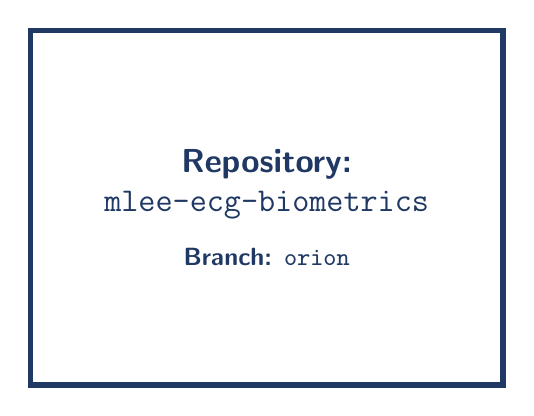
\begin{tikzpicture}
    \node[draw=bitsnavy, line width=2pt, minimum width=6cm, minimum height=4.5cm,
          text=bitsnavy, align=center, font=\large\bfseries] {Repository:\\\texttt{mlee-ecg-biometrics}\\[2mm]\small Branch: \texttt{orion}};
  \end{tikzpicture}
  \end{center}
  {\small Instructor: Dr. Ritesh Vyas\\Course: EEE G513, BITS Pilani}
}
\end{subcolumns}

\end{columns}
\end{document}
